%% main.tex — WikiKGQA Challenge @ ISWC 2026
%% Format CEUR-ART (une colonne), langue française
\documentclass[]{ceurart}

\sloppy

%% --- Langue française ---
\usepackage[french]{babel}
\usepackage[T1]{fontenc}
\usepackage{lmodern}

%% --- Tables et figures ---
\usepackage{booktabs}
\usepackage{tabularx}
\usepackage{multirow}
\usepackage{array}
\usepackage{url}
\usepackage{xcolor}
\usepackage{listings}
\usepackage{graphicx}
\graphicspath{{images/}}
\usepackage{siunitx}
\sisetup{group-separator={\,},output-decimal-marker={,}}
\lstset{
  basicstyle=\ttfamily\footnotesize,
  breaklines=true,
  showstringspaces=false,
  frame=single,
  framerule=0.3pt,
  rulecolor=\color{gray!50},
  columns=fullflexible,
  keepspaces=true,
  belowskip=0.4em,
  aboveskip=0.4em,
}

\begin{document}

\copyrightyear{2026}
\copyrightclause{Copyright for this paper by its authors.
  Use permitted under Creative Commons License Attribution 4.0 International (CC BY 4.0).}

\conference{WikiKGQA Challenge @ ISWC 2026: International Semantic Web Conference, October 2026, Nara, Japan}

\title{Génération de SPARQL sur Wikidata par few-shot prompting et sélection guidée par exécution~: participation au défi WikiKGQA~@~ISWC~2026}

\tnotemark[1]
\tnotetext[1]{Papier de participation au défi WikiKGQA~@~ISWC~2026, pistes \texttt{en-with-mentions} et \texttt{es-with-mentions}.}

\author[1]{Kenmegne Fokam Emeric Cyrille}[%
orcid=0009-0000-0000-0001,
email=kenmegne.fokam@facsciences-uy1.cm,
]
\cormark[1]

\author[1]{Tela Tela Gilbert Ebenezer}[%
orcid=0009-0000-0000-0002,
email=telaebenezer@gmail.com,
]

\address[1]{Université de Yaoundé~I, Faculté des Sciences, BP 812 Yaoundé, Cameroun}

\cortext[1]{Auteur correspondant.}

\begin{abstract}
Nous décrivons notre participation aux deux pistes \emph{with-mentions} (EN, ES) du défi WikiKGQA~@~ISWC~2026, qui demande de traduire des questions en langue naturelle en requêtes SPARQL exécutables sur un sous-ensemble de Wikidata. Notre pipeline enchaîne quatre étapes~: retrieval TF-IDF de trois exemples similaires, prompt \emph{few-shot}, génération de cinq candidats à températures mixtes (un déterministe, quatre à 0{,}7), et sélection du premier candidat renvoyant un résultat non vide sur l'\emph{endpoint}. Sur le développement (100~questions par langue), nous obtenons F1~macro~=~0{,}634 (EN) et 0{,}607 (ES). Sur le test officiel Codabench (75~questions par langue), les scores sont 0{,}65 (EN) et 0{,}63 (ES). Deux catégories concentrent les échecs~: les questions typées en \emph{«~which~/~qué~»} qui reposent sur la chaîne \texttt{P31/P279*} incomplète sur l'\emph{endpoint}, et les requêtes \texttt{COUNT} pour lesquelles le LLM omet fréquemment l'agrégat. L'ensemble n'utilise que des LLM ouverts (\texttt{gpt-oss-120b}, \texttt{llama-3.3-70b}) via le \emph{free tier} de Groq Cloud.
\end{abstract}

\begin{keywords}
  Knowledge Graph Question Answering \sep
  Text-to-SPARQL \sep
  Wikidata \sep
  Large Language Models \sep
  In-context Learning \sep
  QAWiki
\end{keywords}

\maketitle

%==============================================================================
\section{Introduction}
\label{sec:intro}
%==============================================================================

Le \emph{Knowledge Graph Question Answering} (KGQA) permet d'interroger un graphe RDF en langue naturelle. L'intérêt est double~: rendre un graphe ouvert comme Wikidata~\cite{vrandecic2014wikidata} accessible sans SPARQL, et produire une couche de raisonnement vérifiable — la requête générée peut être inspectée, corrigée et rejouée, contrairement aux réponses opaques d'un LLM. Deux difficultés dominent~: la désambiguïsation des mentions vers les Q-identifiants, et la traduction de la structure logique de la question en un motif de graphe correct (propriétés, agrégats, filtres, jointures), le tout en contexte multilingue.

Le défi WikiKGQA~@~ISWC~2026 fournit à cet effet \num{497}~paires bilingues (EN~/~ES) question–SPARQL adossées au corpus QAWiki, un \emph{endpoint} QLever~\cite{bast2017qlever} servant une vue simplifiée de Wikidata figée pour toute la durée du défi, et une évaluation \emph{online} sur Codabench utilisant la F1~macro QALD~\cite{usbeck2017qald}. Nous participons aux deux pistes \emph{with-mentions}, où les Q-identifiants des entités mentionnées sont fournis avec la question — ce qui isole la difficulté de la génération de requête.

\paragraph{Contributions.}
\begin{enumerate}
  \item Un pipeline en quatre étapes (retrieval TF-IDF, \emph{few-shot prompting}, génération multi-candidate, sélection guidée par exécution) entièrement construit sur des LLM ouverts.
  \item Une évaluation dev et test des deux pistes \emph{with-mentions}, avec F1~macro respectivement 0{,}634~/~0{,}607 et 0{,}65~/~0{,}63.
  \item Une analyse d'erreurs structurée qui isole deux catégories résistantes~: questions typées (\emph{which~/~qué}) et requêtes \texttt{COUNT}.
  \item Un retour d'expérience sur un bug de \emph{parsing} des mentions découvert en soumission, dont la correction a fait passer notre score EN de 0{,}11 à 0{,}65.
\end{enumerate}

%==============================================================================
\section{Travaux connexes}
\label{sec:related}
%==============================================================================

\paragraph{KGQA et QALD.} La série QALD~\cite{usbeck2017qald}, migrée sur Wikidata avec QALD-10, a fixé le protocole d'évaluation (F1 macro sur l'union des réponses). Les approches classiques par \emph{parsers} supervisés ou \emph{templates} obtiennent de bons résultats sur des distributions vues mais généralisent mal aux reformulations nouvelles.

\paragraph{Text-to-SPARQL.} La génération seq2seq (T5, BART \emph{fine-tuné}) produit une syntaxe correcte mais souffre d'IRI hallucinées~: le modèle génère des propriétés plausibles qui n'existent pas dans le graphe cible. Les décodages à grammaire contrainte rétablissent la validité syntaxique mais pas la satisfiabilité sémantique — c'est précisément la faille que notre sélection par exécution comble.

\paragraph{LLM et \emph{in-context learning}.} Depuis \cite{brown2020gpt3}, plusieurs travaux~\cite{li2023fewshot,jiang2023structgpt} montrent qu'un LLM instruit produit des requêtes SPARQL compétitives à partir de quelques exemples. KAPING~\cite{baek2023kaping} injecte le voisinage du graphe~; ChatKBQA~\cite{luo2024chatkbqa} et DecAF~\cite{yu2023decaf} décomposent le processus. Nous héritons du principe \emph{few-shot} guidé par retrieval, mais choisissons un retrieveur non appris (TF-IDF, \cite{salton1988term}) par souci de reproductibilité.

\paragraph{Auto-cohérence.} Wang \emph{et al.}~\cite{wang2022selfconsistency} popularisent le vote sur plusieurs échantillons~; Self-Refine~\cite{madaan2023selfrefine} et Reflexion~\cite{shinn2023reflexion} y ajoutent une critique automatique. Notre sélection guidée par exécution s'inscrit dans cette famille en évacuant l'étape critique~: l'\emph{endpoint} lui-même joue le rôle d'oracle.

%==============================================================================
\section{Tâche et données}
\label{sec:task}
%==============================================================================

Le défi demande, pour chaque question en langue naturelle, une requête SPARQL exécutable et l'ensemble des réponses attendues (Q-identifiants pour \texttt{SELECT}, valeur booléenne pour \texttt{ASK}, entier pour \texttt{COUNT}). Quatre pistes sont proposées~: deux avec mentions d'entités fournies (EN et ES), deux sans. Nous couvrons les deux pistes \emph{with-mentions}.

Le corpus QAWiki est distribué au format JSON dérivé du schéma QALD. Chaque item réunit un identifiant, la question bilingue, la liste des mentions (label~+~Q-id), la SPARQL de référence et les réponses (Fig.~\ref{fig:dataset}). La version 2026.2 contient \num{497}~questions, réparties en \num{317}~train~/~\num{100}~dev~/~\num{80}~test (75~effectivement scorées). Le graphe cible est servi par un \emph{endpoint} QLever~\cite{bast2017qlever} spécifique au défi (\texttt{backend.wikikgqa.skynet.coypu.org})~; contrairement à l'\emph{endpoint} public de Wikidata, la vue est \emph{simplifiée} et certaines hiérarchies (notamment \texttt{P31/P279*}) sont incomplètes. Une requête syntaxiquement parfaite peut donc renvoyer un résultat vide simplement parce que la propriété n'est pas matérialisée.

\begin{figure}[h]
\centering
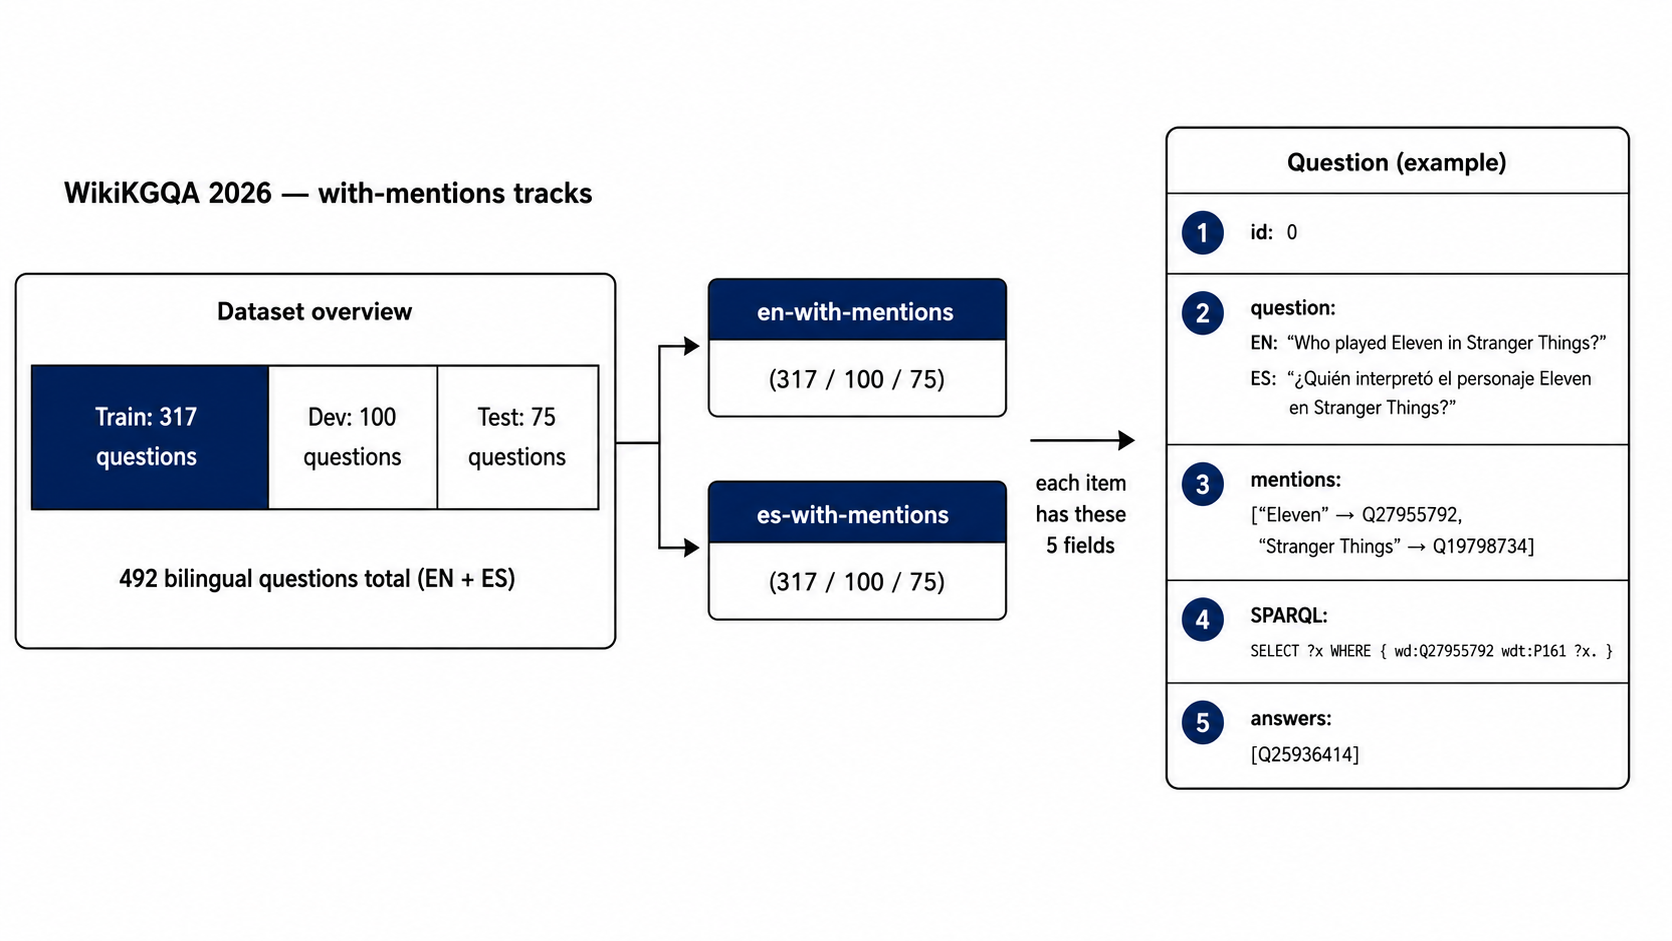
\includegraphics[width=0.9\linewidth]{data.png}
\caption{Format d'un item du corpus QAWiki~: question bilingue, mentions d'entités avec Q-id, requête SPARQL de référence, réponses attendues.}
\label{fig:dataset}
\end{figure}

La métrique officielle est la F1~macro QALD~\cite{usbeck2017qald}~: pour chaque question, $\mathrm{F1}_q = 2PR/(P+R)$ où $P$ et $R$ portent sur l'ensemble des réponses~; le score global est la moyenne $|Q|^{-1}\sum_q \mathrm{F1}_q$. Nous rapportons aussi le nombre de questions parfaites ($\mathrm{F1}_q=1$) et nulles ($\mathrm{F1}_q=0$).

%==============================================================================
\section{Système proposé}
\label{sec:method}
%==============================================================================

\subsection{Vue d'ensemble}

La figure~\ref{fig:pipeline} synthétise notre pipeline, désigné P3. Entrée~: une question et ses mentions. Sortie~: une requête SPARQL et son ensemble de réponses. Le flux est linéaire, sans agent ni re-ranker appris.

\begin{figure}[h]
\centering
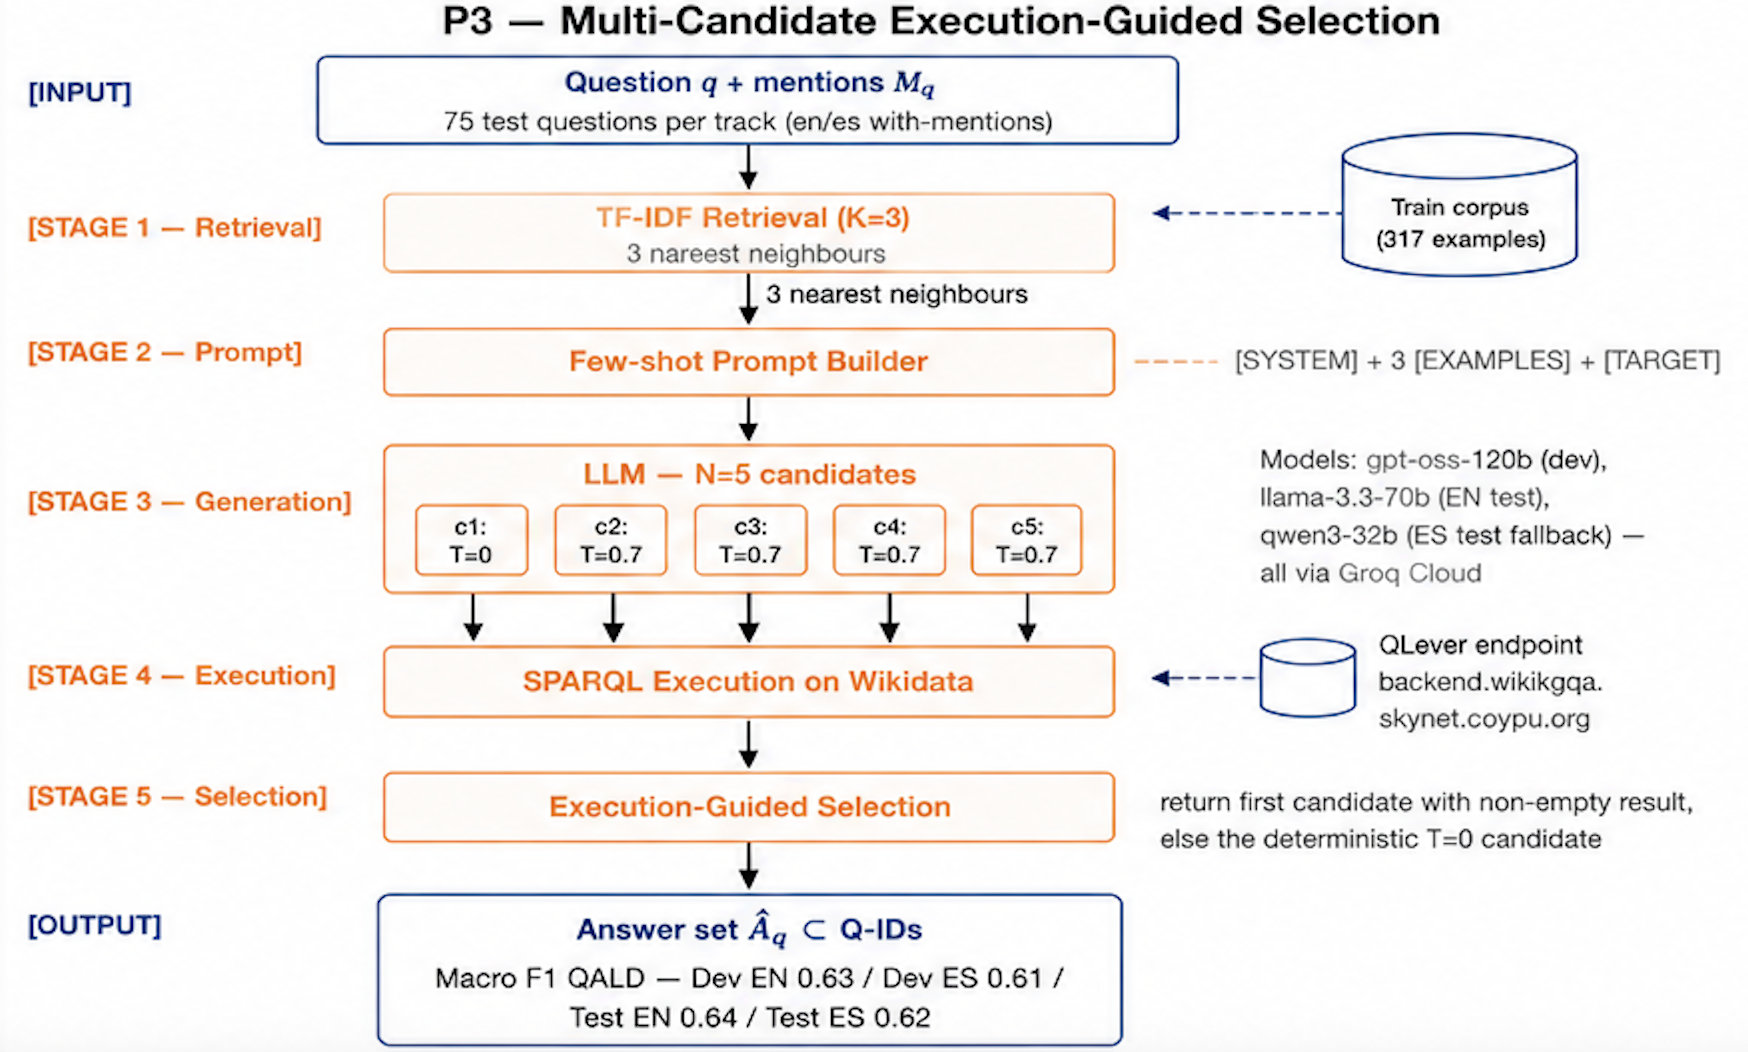
\includegraphics[width=0.78\linewidth]{solution.png}
\caption{Pipeline P3. (1)~Retrieval TF-IDF des trois voisins les plus proches~; (2)~prompt \emph{few-shot}~; (3)~cinq candidats SPARQL (un à $T=0$, quatre à $T=0{,}7$)~; (4)~exécution sur l'\emph{endpoint}~; (5)~sélection du premier candidat non vide.}
\label{fig:pipeline}
\end{figure}

\subsection{Retrieval et construction du prompt}

Pour chaque question cible $q$, nous récupérons les $K=3$~voisins les plus proches dans le train au sens du cosinus TF-IDF~\cite{salton1988term}~: $\mathrm{sim}(q,q') = v_q\cdot v_{q'} / (\|v_q\|\|v_{q'}\|)$, avec $n$-grammes de mots ($n\in\{1,2\}$). Une heuristique légère infère le type cible (\texttt{ASK}, \texttt{COUNT}, \texttt{SELECT}) à partir des interrogatifs et privilégie les voisins de même type. L'entraînement du vectoriseur prend moins d'une seconde sur les \num{317}~questions du train et ne dépend d'aucun modèle externe.

Le prompt enchaîne trois blocs~: (i)~une consigne système («~\emph{You are an expert at generating SPARQL for Wikidata. Output ONLY the query inside a fenced code block. No PREFIX.}~»), (ii)~les $K$~exemples formatés en triplets \texttt{(question, mentions, SPARQL)} chacun clos par un \emph{fenced block} \texttt{```sparql~\dots~```}, (iii)~la question cible et ses mentions sous le même format, terminée par \texttt{SPARQL:} pour amorcer la génération. Les déclarations \texttt{PREFIX} sont volontairement omises et ajoutées automatiquement à l'exécution~; cela raccourcit le prompt et évite les préfixes hallucinés.

\subsection{Génération multi-candidate et sélection par exécution}
\label{sec:execution}

Nous interrogeons le LLM $N=5$~fois pour la même question. Le premier appel est à $T=0$ (pari le plus probable), les quatre suivants à $T=0{,}7$ (diversification). Chaque candidat est extrait de son bloc de code, préfixé automatiquement par les \texttt{PREFIX} de Wikidata, puis soumis à l'\emph{endpoint} via HTTP POST (\emph{timeout} 30~s, \emph{retry} adaptatif sur 429/5xx respectant le \texttt{Retry-After} de Groq). La règle de sélection est simple~: nous renvoyons les réponses du premier candidat qui produit au moins une ligne. Si tous les candidats renvoient vide, nous conservons la sortie déterministe — ce qui couvre les rares cas où la réponse \emph{gold} est effectivement vide (\texttt{ASK} négatif, \texttt{SELECT} avec \texttt{MINUS}).

L'intuition~: le LLM connaît la structure publique de Wikidata mais ignore la vue simplifiée du défi. Une paraphrase entre candidats permet souvent de trouver un motif satisfaisable~; l'\emph{endpoint} joue le rôle d'oracle en séparant les requêtes vides des exploitables.

\subsection{Pré- et post-traitement}

Trois garde-fous complètent le pipeline. (i)~L'extracteur de mentions utilise la regex permissive \texttt{(Q\textbackslash d+)} qui accepte les URI complètes (\texttt{http://\dots/Q42}) comme les Q-identifiants nus (\texttt{Q42}) — voir §\ref{sec:results}. (ii)~Si le LLM omet le \emph{fenced block}, un extracteur secondaire capture le premier motif ressemblant à une requête. (iii)~En cas de \emph{timeout} de l'\emph{endpoint}, le candidat est marqué vide et le suivant est essayé (une exception non attrapée causait initialement des chutes silencieuses sur $\sim$3~\% des questions).

Le pipeline ne différencie pas EN et ES au niveau du code~: retrieveur, format du prompt et logique de sélection sont identiques. TF-IDF construit toutefois deux vocabulaires distincts (un par langue), et nous observons que la diversité inter-températures du LLM est plus faible en ES qu'en EN (§\ref{sec:erranalysis}).

%==============================================================================
\section{Protocole expérimental}
\label{sec:setup}
%==============================================================================

Nous utilisons les splits officiels (\num{317} train~/~\num{100} dev~/~\num{75} test) et évaluons avec la F1~macro QALD (§\ref{sec:task}). Deux LLM ouverts servent nos expériences~: \texttt{openai/gpt-oss-120b}~\cite{openai2025gptoss} et \texttt{meta-llama/llama-3.3-70b-versatile}, accessibles via le \emph{free tier} de Groq Cloud~\cite{groq2024} (200~k et 100~k tokens/jour). Hyperparamètres~: $K=3$, $N=5$, températures $(0{,}0;0{,}7;0{,}7;0{,}7;0{,}7)$, \texttt{max\_tokens=2048}, pause 6~s entre appels. Aucun \emph{fine-tuning}~; le train sert uniquement à peupler l'index TF-IDF.

Le baseline principal est la variante \emph{single-shot} de P3 (N=1, seul le candidat déterministe est produit), qui isole l'apport de la génération multi-candidate. Un \emph{dev pass} complet prend 15--20~min sur un ordinateur portable sans GPU, la charge d'inférence étant reportée sur Groq. Coût monétaire nul.

Un pré-test a vérifié que notre implémentation locale du scorer reproduit exactement le score renvoyé par Codabench sur les soumissions dev, ce qui permet d'itérer localement avant chaque upload.

%==============================================================================
\section{Résultats}
\label{sec:results}
%==============================================================================

\subsection{Résultats dev et test}

La table~\ref{tab:main} rassemble les scores sur le développement et le test officiel Codabench.

\begin{table}[h]
\centering
\caption{F1 macro sur dev (100~questions) et test (75~questions) des deux pistes \emph{with-mentions}. \emph{Single-shot} sert de borne inférieure (candidat $T=0$ seul).}
\label{tab:main}
\begin{tabular}{llccc}
\toprule
Piste & Méthode & F1 macro & Parfait & Nul \\
\midrule
EN dev & Single-shot (N=1)                             & 0{,}5524 & 52 & 40 \\
EN dev & P3 (multi-candidate + exécution)             & 0{,}6342 & 60 & 31 \\
ES dev & Single-shot (N=1)                             & 0{,}5914 & 55 & 37 \\
ES dev & P3 (multi-candidate + exécution)             & 0{,}6073 & 56 & 34 \\
\midrule
EN test & P3 (bug regex mentions)                      & 0{,}11 & — & — \\
EN test & P3 (regex corrigée, llama-3.3-70b)           & 0{,}65 & — & — \\
ES test & P3 (regex corrigée, gpt-oss-120b)            & 0{,}63 & — & — \\
\bottomrule
\end{tabular}
\end{table}

Le multi-candidate apporte +8{,}2~F1 en EN et seulement +1{,}6 en ES. L'asymétrie s'explique par la borne inférieure~: en ES le candidat déterministe seul obtient déjà 0{,}59, ce qui laisse moins de marge de rattrapage. Les scores test (0{,}65~/~0{,}63) sont en parité étroite avec le dev, ce qui indique l'absence de surapprentissage à la distribution de développement.

\subsection{Bug de \emph{parsing} des mentions}

Notre première soumission EN a obtenu 0{,}11 sur Codabench alors que le dev culminait à 0{,}63. Le format des annotations diffère entre partitions~: le dev fournit des URI complètes (\texttt{http://www.wikidata.org/entity/Q19798734}), le test des Q-identifiants nus (\texttt{Q19798734}). Notre extracteur exigeait le slash final, rejetait silencieusement les identifiants du test, et le LLM recevait donc un prompt sans aucun Q-id — d'où l'hallucination systématique d'entités erronées. Le correctif (relâchement de la regex à \texttt{(Q\textbackslash d+)}) a rétabli la performance attendue. Sur la piste ES, une saturation du quota TPD de \texttt{gpt-oss-120b} nous a contraints à effectuer les 12~dernières questions avec \texttt{qwen3-32b}~; l'homogénéité du score suggère que la performance du pipeline est dominée par les choix structurels (retrieval, format du prompt, extraction des mentions) plutôt que par le choix précis du LLM ouvert.

\subsection{Sensibilité du retrieveur}

Le chevauchement Jaccard entre les voisins top-3 de TF-IDF et ceux de trois encodeurs neuronaux (\texttt{all-MiniLM-L6-v2}, \texttt{bge-small-en-v1.5}, \texttt{bge-m3}~\cite{chen2024bge,reimers2019sbert}) tourne autour de 0{,}20. Un remplacement par un retrieveur neuronal reconstruirait donc massivement le contexte few-shot, ce qui constitue notre principale piste d'amélioration.

%==============================================================================
\section{Analyse d'erreurs et discussion}
\label{sec:erranalysis}
%==============================================================================

Nous croisons les prédictions de P3 avec le type de requête généré, le mot interrogatif, le nombre de mentions et la longueur de la question.

\subsection{Type de requête et mot interrogatif}

La table~\ref{tab:bytypeinterr} regroupe les deux vues. Les \texttt{COUNT} sous-performent (0{,}33~EN, 0{,}52~ES)~: le mode d'échec récurrent est l'oubli de l'agrégat — le LLM produit \texttt{SELECT ?c WHERE \{~\dots~\}} au lieu de \texttt{SELECT (COUNT(?c) AS ?n) WHERE \{~\dots~\}}. À l'inverse, les \texttt{ASK} en espagnol atteignent 0{,}90~: les formulations oui/non ES (\emph{«~¿Es~\ldots ?~»}, \emph{«~¿Tiene~\ldots ?~»}) sont plus contraintes qu'en EN.

\begin{table}[h]
\centering
\caption{Performance par type de requête (bloc supérieur) et par mot interrogatif dominant (bloc inférieur), dev EN et ES.}
\label{tab:bytypeinterr}
\begin{tabular}{lcccccc}
\toprule
 & \multicolumn{3}{c}{EN} & \multicolumn{3}{c}{ES} \\
\cmidrule(lr){2-4}\cmidrule(lr){5-7}
Catégorie & $n$ & F1 & Nul & $n$ & F1 & Nul \\
\midrule
\multicolumn{7}{l}{\emph{Par type de requête}} \\
SELECT   & 81 & 0{,}647 & 23 & 74 & 0{,}608 & 24 \\
ASK      & 13 & 0{,}692 &  4 & 10 & 0{,}900 &  1 \\
COUNT    &  6 & 0{,}333 &  4 & 13 & 0{,}520 &  6 \\
\midrule
\multicolumn{7}{l}{\emph{Par mot interrogatif dominant}} \\
which~/~qué       & 32 & 0{,}425 & 15 & 39 & 0{,}470 & 16 \\
what~/~cuál       & 23 & 0{,}701 &  6 &  9 & 0{,}667 &  3 \\
who~/~quién       & 13 & 0{,}822 &  1 & 13 & 0{,}800 &  2 \\
when~/~cuándo     &  9 & 1{,}000 &  0 &  9 & 0{,}889 &  1 \\
how-many~/~cuántos&  5 & 0{,}200 &  4 & 10 & 0{,}400 &  6 \\
yes-no            & 13 & 0{,}692 &  4 & 11 & 0{,}818 &  2 \\
\bottomrule
\end{tabular}
\end{table}

L'observation la plus nette est structurellement identique dans les deux langues~: une seule catégorie d'interrogatifs concentre la moitié des nuls. En EN, les \emph{«~which~»} (32~\% du dev) totalisent 15~nuls sur 31~; en ES, les \emph{«~qué~»} (39~\%) totalisent 16~nuls sur 34. Ces deux catégories partagent la même structure~: filtrer un ensemble par leur type, ce qui passe par la chaîne \texttt{?x wdt:P31/wdt:P279* wd:Qtype}. Cette fermeture transitive est incomplète sur l'\emph{endpoint} du défi~; le LLM génère la chaîne plausible mais l'exécution renvoie zéro ligne. À l'inverse, les questions courtes reposant sur une propriété directe (\emph{when~/~cuándo}, \emph{who~/~quién}) sont quasi-parfaites, car \texttt{P569} (date de naissance) et \texttt{P161} (distribution) sont bien matérialisées.

\subsection{Effet du nombre de mentions et de la longueur, et rentabilité du multi-candidate}

Deux gradients complémentaires apparaissent (Table~\ref{tab:covariates})~: (i)~la F1 chute de 0{,}30~point en EN (0{,}23 en ES) entre les questions à 2~mentions et celles à 3+~; (ii)~elle chute de 0{,}16 en EN (0{,}19 en ES) entre les questions courtes ($\leq 6$~mots) et moyennes (7--10~mots). Ces effets convergent avec la catégorie \emph{«~which~/~qué~»}, plus longue et plus contrainte en moyenne.

La distribution des essais (Table~\ref{tab:covariates}, bloc inférieur) éclaire le mécanisme du multi-candidate. Trois régimes~: (a)~\emph{immédiat} (essai~1)~: 75~\% des questions résolues au premier tir avec F1 moyenne~$>0{,}73$~; (b)~\emph{rattrapage} (essais 2--4)~: efficace en EN (7 gains à F1~$\geq 0{,}73$), marginal en ES~; (c)~\emph{épuisé} (essai~5, tous précédents vides)~: rien récupéré (F1 moyenne 0{,}13 en EN, 0{,}00 en ES). Ces 16--18~questions par langue correspondent au profil homogène des \texttt{P31/P279*} et exigent un mécanisme différent du multi-candidate à températures.

\begin{table}[h]
\centering
\caption{Trois vues complémentaires du dev~: nombre de mentions (haut), longueur en mots (milieu), et essais nécessaires pour obtenir une réponse non vide (bas).}
\label{tab:covariates}
\begin{tabular}{lcccccc}
\toprule
 & \multicolumn{3}{c}{EN} & \multicolumn{3}{c}{ES} \\
\cmidrule(lr){2-4}\cmidrule(lr){5-7}
Catégorie & $n$ & F1 & Nul & $n$ & F1 & Nul \\
\midrule
\multicolumn{7}{l}{\emph{Nombre de mentions}} \\
2   & 16 & 0{,}886 &  1 & 29 & 0{,}770 &  5 \\
3+  & 84 & 0{,}586 & 30 & 71 & 0{,}541 & 29 \\
\midrule
\multicolumn{7}{l}{\emph{Longueur (mots)}} \\
0--6   & 39 & 0{,}732 &  8 & 30 & 0{,}736 &  6 \\
7--10  & 54 & 0{,}571 & 20 & 58 & 0{,}543 & 24 \\
11--14 &  7 & 0{,}571 &  3 & 12 & 0{,}596 &  4 \\
\midrule
\multicolumn{7}{l}{\emph{Essais nécessaires} (F1 moyenne)} \\
1 essai   & 75 & 0{,}737 & — & 74 & 0{,}799 & — \\
2--4      &  7 & 0{,}870 & — &  5 & 0{,}304 & — \\
5 (vides) & 16 & 0{,}125 & — & 18 & 0{,}000 & — \\
\bottomrule
\end{tabular}
\end{table}

\subsection{Discussion}

\paragraph{Différences EN \emph{vs} ES.} Le candidat déterministe est plus souvent correct en ES (55 parfaits contre 52 en EN)~; le rattrapage multi-candidate y est en revanche nettement moins efficace, les températures 0{,}7 produisant des reformulations plus proches les unes des autres. La catégorie dominante d'échecs est isomorphe entre les deux langues (\emph{which} $\leftrightarrow$ \emph{qué}), pour la même raison technique.

\paragraph{Limites et pistes.} Notre méthode ignore la structure réelle du graphe~: elle génère à partir de la mémoire paramétrique du LLM et corrige a posteriori par exécution, ce qui produit une catégorie d'échecs prévisibles (chaînes transitives non matérialisées). TF-IDF rate par ailleurs les paraphrases (chevauchement Jaccard $\approx 0{,}2$, §\ref{sec:results}). Trois directions ciblées~: un retrieveur neuronal (\texttt{bge-m3}) pour les paraphrases~; un profilage léger de l'\emph{endpoint} (\texttt{SELECT ?p (COUNT(?o) AS ?n)} par entité) pour fournir au LLM la liste des propriétés effectivement disponibles~; un tour de raffinement conditionnel à la Self-Refine~\cite{madaan2023selfrefine} sur le régime \emph{épuisé} de la Table~\ref{tab:covariates}.

%==============================================================================
\section{Conclusion}
\label{sec:conclusion}
%==============================================================================

Nous avons présenté notre participation aux deux pistes \emph{with-mentions} du défi WikiKGQA~@~ISWC~2026. Le pipeline enchaîne retrieval TF-IDF, prompt \emph{few-shot}, génération de cinq candidats à températures mixtes et sélection guidée par l'exécution. Il atteint F1~macro~=~0{,}634 (EN) et 0{,}607 (ES) sur le développement, 0{,}65 (EN) et 0{,}63 (ES) sur le test officiel Codabench, en utilisant uniquement des LLM ouverts. L'analyse d'erreurs isole deux catégories résistantes — questions typées \emph{which~/~qué} et requêtes \texttt{COUNT} — et suggère trois pistes ciblées (retrieveur neuronal, profilage du \emph{endpoint}, raffinement conditionnel). Une leçon opérationnelle mérite d'être rappelée~: un simple désalignement du format des mentions entre dev et test a fait chuter notre score EN de 0{,}65 à 0{,}11 avant qu'une correction d'une seule regex ne rétablisse la performance. Le code, les \emph{traces} et les fichiers de soumission accompagnent ce papier pour reproductibilité complète.

\paragraph{Disponibilité.} Code, scripts d'évaluation, \emph{traces} JSON et archives Codabench sont disponibles à \url{https://github.com/tela-ebenezer/wikikgqa-iswc2026}. Le corpus QAWiki (v2026.2) est distribué sous licence CC~BY~4.0 sur Zenodo.

\paragraph{Usage d'outils d'IA générative.} La génération des requêtes SPARQL au c\oe{}ur de la méthode mobilise deux LLM ouverts (\texttt{gpt-oss-120b}, \texttt{llama-3.3-70b}) via Groq~: c'est le sujet même du défi. Un outil d'assistance a par ailleurs été utilisé pour la reformulation et la vérification orthographique~; tout le contenu scientifique, l'analyse, le code, les tableaux et les affirmations finales relèvent de la responsabilité des auteurs.

%==============================================================================
\bibliography{main}
%==============================================================================

\end{document}
